\documentclass[tikz]{standalone}
\usepackage{pgfplots}
\pgfplotsset{compat=1.15}
\usepackage{mathrsfs}
\usetikzlibrary{arrows,calc}
\usepackage{tkz-euclide}
\pagestyle{empty}

\definecolor{AngleClr}{rgb}{0,0.39215686274509803,0}
\definecolor{ShapeClr}{rgb}{0.6,0.2,0}
\definecolor{BlueClr}{RGB}{90, 132, 191}

\begin{document}

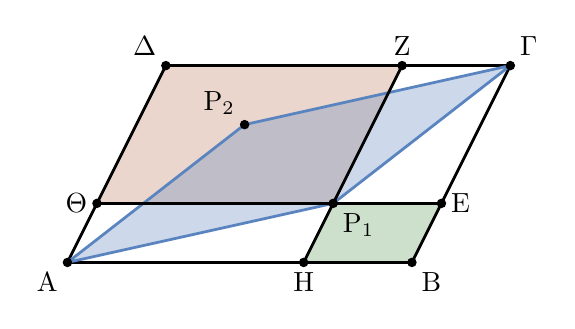
\begin{tikzpicture}[scale=1.25]
\tkzSetUpLine[line width=1pt,color=black]
\tkzSetUpPoint[fill=black]

\tkzDefPoints{0/0/A,3.5/0/B,1/2/D,4.5/2/C,2.7/0.6/P1}

\tkzInterLL(A,C)(B,D) \tkzGetPoint{O}
\tkzDefPointsBy[symmetry=center O](P1){P2}

\tkzDefLine[parallel=through P1](B,C) \tkzGetPoint{x}
\tkzDefLine[parallel=through P1](A,B) \tkzGetPoint{y}

\tkzInterLL(P1,x)(A,B) \tkzGetPoint{H}
\tkzInterLL(P1,x)(C,D) \tkzGetPoint{Z}

\tkzInterLL(P1,y)(A,D) \tkzGetPoint{Th}
\tkzInterLL(P1,y)(B,C) \tkzGetPoint{E}

\tkzFillPolygon[fill=white](A,B,C,D)
\tkzFillPolygon[fill=ShapeClr,fill opacity=0.2](P1,Z,D,Th)
\tkzFillPolygon[fill=AngleClr,fill opacity=0.2](H,B,E,P1)
\tkzFillPolygon[fill=BlueClr,fill opacity=0.3](A,P1,C,P2)
\tkzDrawPolygon[color=black](A,B,C,D)
\tkzDrawPolygon[color=BlueClr](A,P1,C,P2)

\tkzDrawSegments(E,Th Z,H);

\tkzDrawPoints[size=3](A,B,C,D,P1,P2,E,Z,H,Th)
\tkzLabelPoint[below left](A){$\rm A$}
\tkzLabelPoint[below right](B){$\rm B$}
\tkzLabelPoint[above right](C){$\rm \Gamma$};
\tkzLabelPoint[above left](D){$\rm \Delta$};
\tkzLabelPoint[below right](P1){${\rm P}_1$};
\tkzLabelPoint[above left](P2){${\rm P}_2$};

\tkzLabelPoint[right](E){$\rm E$};
\tkzLabelPoint[above](Z){$\rm Z$};
\tkzLabelPoint[below](H){$\rm H$};
\tkzLabelPoint[left](Th){$\rm \Theta$};

\end{tikzpicture}

\end{document}
